\documentclass[preprint, 3p,
authoryear]{elsarticle} %review=doublespace preprint=single 5p=2 column
%%% Begin My package additions %%%%%%%%%%%%%%%%%%%

\usepackage[hyphens]{url}

  \journal{Reviews in Aquaculture} % Sets Journal name

\usepackage{lineno} % add
  \linenumbers % turns line numbering on

\usepackage{graphicx}
%%%%%%%%%%%%%%%% end my additions to header

\usepackage[T1]{fontenc}
\usepackage{lmodern}
\usepackage{amssymb,amsmath}
\usepackage{ifxetex,ifluatex}
\usepackage{fixltx2e} % provides \textsubscript
% use upquote if available, for straight quotes in verbatim environments
\IfFileExists{upquote.sty}{\usepackage{upquote}}{}
\ifnum 0\ifxetex 1\fi\ifluatex 1\fi=0 % if pdftex
  \usepackage[utf8]{inputenc}
\else % if luatex or xelatex
  \usepackage{fontspec}
  \ifxetex
    \usepackage{xltxtra,xunicode}
  \fi
  \defaultfontfeatures{Mapping=tex-text,Scale=MatchLowercase}
  \newcommand{\euro}{€}
\fi
% use microtype if available
\IfFileExists{microtype.sty}{\usepackage{microtype}}{}

\ifxetex
  \usepackage[setpagesize=false, % page size defined by xetex
              unicode=false, % unicode breaks when used with xetex
              xetex]{hyperref}
\else
  \usepackage[unicode=true]{hyperref}
\fi
\hypersetup{breaklinks=true,
            bookmarks=true,
            pdfauthor={},
            pdftitle={Sources of nutrients, their variability and contribution to the total input into aquaponic systems},
            colorlinks=false,
            urlcolor=blue,
            linkcolor=magenta,
            pdfborder={0 0 0}}

\setcounter{secnumdepth}{5}
% Pandoc toggle for numbering sections (defaults to be off)


% tightlist command for lists without linebreak
\providecommand{\tightlist}{%
  \setlength{\itemsep}{0pt}\setlength{\parskip}{0pt}}


% Pandoc citation processing
\newlength{\cslhangindent}
\setlength{\cslhangindent}{1.5em}
\newlength{\csllabelwidth}
\setlength{\csllabelwidth}{3em}
\newlength{\cslentryspacingunit} % times entry-spacing
\setlength{\cslentryspacingunit}{\parskip}
% for Pandoc 2.8 to 2.10.1
\newenvironment{cslreferences}%
  {}%
  {\par}
% For Pandoc 2.11+
\newenvironment{CSLReferences}[2] % #1 hanging-ident, #2 entry spacing
 {% don't indent paragraphs
  \setlength{\parindent}{0pt}
  % turn on hanging indent if param 1 is 1
  \ifodd #1
  \let\oldpar\par
  \def\par{\hangindent=\cslhangindent\oldpar}
  \fi
  % set entry spacing
  \setlength{\parskip}{#2\cslentryspacingunit}
 }%
 {}
\usepackage{calc}
\newcommand{\CSLBlock}[1]{#1\hfill\break}
\newcommand{\CSLLeftMargin}[1]{\parbox[t]{\csllabelwidth}{#1}}
\newcommand{\CSLRightInline}[1]{\parbox[t]{\linewidth - \csllabelwidth}{#1}\break}
\newcommand{\CSLIndent}[1]{\hspace{\cslhangindent}#1}

\usepackage[utf8]{inputenc}

\usepackage{setspace}
\doublespacing

\usepackage[version = 4]{mhchem}

% TABLES
\usepackage{tabularx}
\usepackage{booktabs}
\usepackage{rotating}

% SIUNITX
\usepackage{siunitx}

\sisetup{separate-uncertainty, multi-part-units = repeat}

\DeclareSIUnit[number-unit-product = {}]\degC{\degreeCelsius}
\DeclareSIUnit[number-unit-product = {}]\p{\percent}
\DeclareSIUnit[number-unit-product = \;]\s{\second}
\DeclareSIUnit[number-unit-product = \;]\min{\minute}
\DeclareSIUnit[number-unit-product = \;]\h{\hour}
\DeclareSIUnit[number-unit-product = \;]\d{\day}
\DeclareSIUnit[number-unit-product = \;]\mm{\milli\meter}
\DeclareSIUnit[number-unit-product = \;]\mL{\milli\liter}
\DeclareSIUnit[number-unit-product = \;]\L{\liter}
\DeclareSIUnit[number-unit-product = \;]\cubicm{\cubic\meter}
\DeclareSIUnit[number-unit-product = \;]\kg{\kilo\gram}
\DeclareSIUnit[number-unit-product = \;]\mg{\milli\gram}
\DeclareSIUnit[number-unit-product = \;]\mgL{\milli\gram\per\liter}
\DeclareSIUnit[number-unit-product = \;]\ug{\micro\gram}
\DeclareSIUnit[number-unit-product = \;]\ugL{\micro\gram\per\liter}
\DeclareSIUnit[number-unit-product = \;]\molL{\mole\per\liter}
\DeclareSIUnit[number-unit-product = \;]\mmolL{\milli\mole\per\liter}
\DeclareSIUnit[number-unit-product = \;]\gmol{\gram\per\mole}

% GLOSSARIES
\usepackage{glossaries}

\newacronym{adc}{ADC}{apparent digestibility coefficient}
\newacronym{cp}{CP}{crude protein}
\newacronym{fr}{FR}{feeding rate}
\newacronym{mle}{MLE}{maximum likelihood estimation}
\newacronym{ras}{RAS}{recirculation aquaculture system}



\begin{document}


\begin{frontmatter}

  \title{Sources of nutrients, their variability and contribution to the
total input into aquaponic systems}
    \author[USB]{Anıl Axel Tellbüscher%
  %
  \fnref{1}}
   \ead{atellbuscher@frov.jcu.cz} 
    \author[USB]{Radek Gebauer%
  %
  \fnref{2}}
   \ead{rgebauer@frov.jcu.cz} 
    \author[USB]{Jan Mráz%
  \corref{cor1}%
  }
   \ead{jmraz@frov.jcu.cz} 
      \affiliation[USB]{}
    \cortext[cor1]{Corresponding author}
    \fntext[1]{This is the first author footnote.}
    \fntext[2]{Another author footnote.}
  
  \begin{abstract}
  Input routes of nutrients into aquaculture and aquaponic systems are
  known, but their contribution to the total nutrient input and the
  variability between locations remains unclear.
  \end{abstract}
    \begin{keyword}
    aquaponics \sep minerals \sep fish feed \sep 
    alkalinity supplements
  \end{keyword}
  
 \end{frontmatter}

\hypertarget{introduction}{%
\section{Introduction}\label{introduction}}

One of the obstacles in the wider adoption of aquaponic systems, the
combination of aquaculture and hydroponics (soilless plant production),
is stated to be the rather complex management of plant nutrients within
the system. While a wide range of ``off-the-shelf'' fertilizer is
available for hydroponics, this is not the case for aquaponic systems.
Developing more efficient and simple nutrient management practices thus
appears to be an opportunity to boost aquaponics.

The most efficient solution for nutrient management would be to monitor
each plant nutrients individually. This would ensure that each
individual nutrient can be supplied in the necessary amount to reach
target concentrations. However, a full-spectrum monitoring of all plant
nutrients is not practical, as it requires expensive equipment and
qualified workforce. Instead, it would be more meaningful to develop a
simple solution that is easily implementable without adding additional
tasks to the working schedule. Optimizing an existing nutrient input is
thus considered as best solution. Though, when optimizing one nutrient
input while not controlling for the others, it is important to consider
the variability that is expected to be introduced by the other sources.
Awareness about the nutrients that run the risk of under- or oversupply
under ``non-average'' conditions is crucial, as this might have adverse
effects on the livestock or plants. Hence, the variability of nutrients
originating from different sources ultimately determines which nutrients
to focus on when optimizing nutrient inputs.

In aquaculture and aquaponics, nutrients enter the system through the
daily ration of feed for the aquatic livestock (hereinafter denoted as
aquafeed), alkalinity supplements used for pH control, and the source
water (Rakocy, Masser, and Losordo 2006; Eck, Körner, and Jijakli 2019;
Robaina et al. 2019). However, even though it is usually stated that
aquafeeds are the most important nutrient source, this claim was never
closer examined and surprisingly little is known about the mass flows of
nutrients in aquaponic systems, although the concept of aquaponics is
already several decades old. The objective of this study is thus to
review the average nutrient concentrations in aquafeeds, alkalinity
supplements, and the source water and assess their variability.

\hypertarget{methodology}{%
\section{Methodology}\label{methodology}}

\hypertarget{rearing-assumptions}{%
\subsection{Rearing assumptions}\label{rearing-assumptions}}

To calculate the proportion contribution of the source water, feed and
alkalinity supplements to the total daily nutrient input in the reviewed
studies, their average daily inputs per volume unit had to be
calculated. For this purpose, initial assumptions with respect to the
husbandry system and rearing conditions were made, as shown in table
\ref{tab:assumptions}. The ASTAF-PRO system (Kloas et al. 2015) was
chosen as model because its sizing is close to reality when comparing it
with results from a recent survey targeting aquaponics production sites
and is well-described in terms of the system components while detailed
information was not provided by the survey results (Pattillo et al.
2022). Consequently, it was assumed that an average \gls{ras} as part of
an aquaponic system would have a total volume of 13 \si{\cubicm}, of
which 7.9 \si{\cubicm} corresponds to the effective volume of the
rearing tanks. The total daily water exchange rate was reported to be
3.8 \si{\p\per\d}. A stocking density of 48.8 \si{\kg\per\cubicm} was
maintained, resulting in an average biomass of 386 \si{\kg}. The feeding
rate was 1.2 \si{\p\per\d}.

\begin{table}
\centering
  \caption{Rearing assumptions for the derivation of mass flows in aquaculture and aquaponic systems.}
  \label{tab:assumptions}
  \begin{tabularx}{\textwidth}{XXXX}
  \toprule
  Parameter & Unit &  Value & Reference \\
  \midrule

  Rearing volume & \si{\cubicm} & \num{10} & [@Pattillo2022] \\
  Total volume & \si{\cubicm} & \num{15} & \\
  Stocking density & \si{\kg\per\cubicm} & \num{25} & \\
  Biomass & \si{\kg} & \num{250} & \\
  Feeding rate & \si{\p\per\d} & \num{2} & \\
  Water exchange rate & \si{\p\per\d} & \num{3} & \\

  \hline

  Total feed input & \si{\kg\per\d} & \num{5} & \\
  Total water input & \si{\cubicm\per\d} & \num{0.45} & \\

  \bottomrule
  \end{tabularx}
\end{table}


\hypertarget{data-collection-and-calculations}{%
\subsection{Data collection and
calculations}\label{data-collection-and-calculations}}

\hypertarget{source-water}{%
\subsubsection{Source water}\label{source-water}}

The daily volume of freshwater introduced into the system (49.8
\si{\p\per\d}) was calculated based on the rearing assumptions. Daily
nutrient inputs via source water were assessed by gathering water
analysis reports from locations all over Europe, covering .

Official reports provided by local authorities and water utilities in
the corresponding municipalities were used to ensure that analyses were
conducted according to accepted laboratory standards.

Collected water analysis reports originated from a total of 20 countries
with 74 analysis reports. The spatial distribution of the analysis
reports is shown in Figure @ref(fig:map\_water).

country distribution of the literature data compared with gathered water
analysis reports is shown in Figure 2.2.

\begin{figure}
\centering
  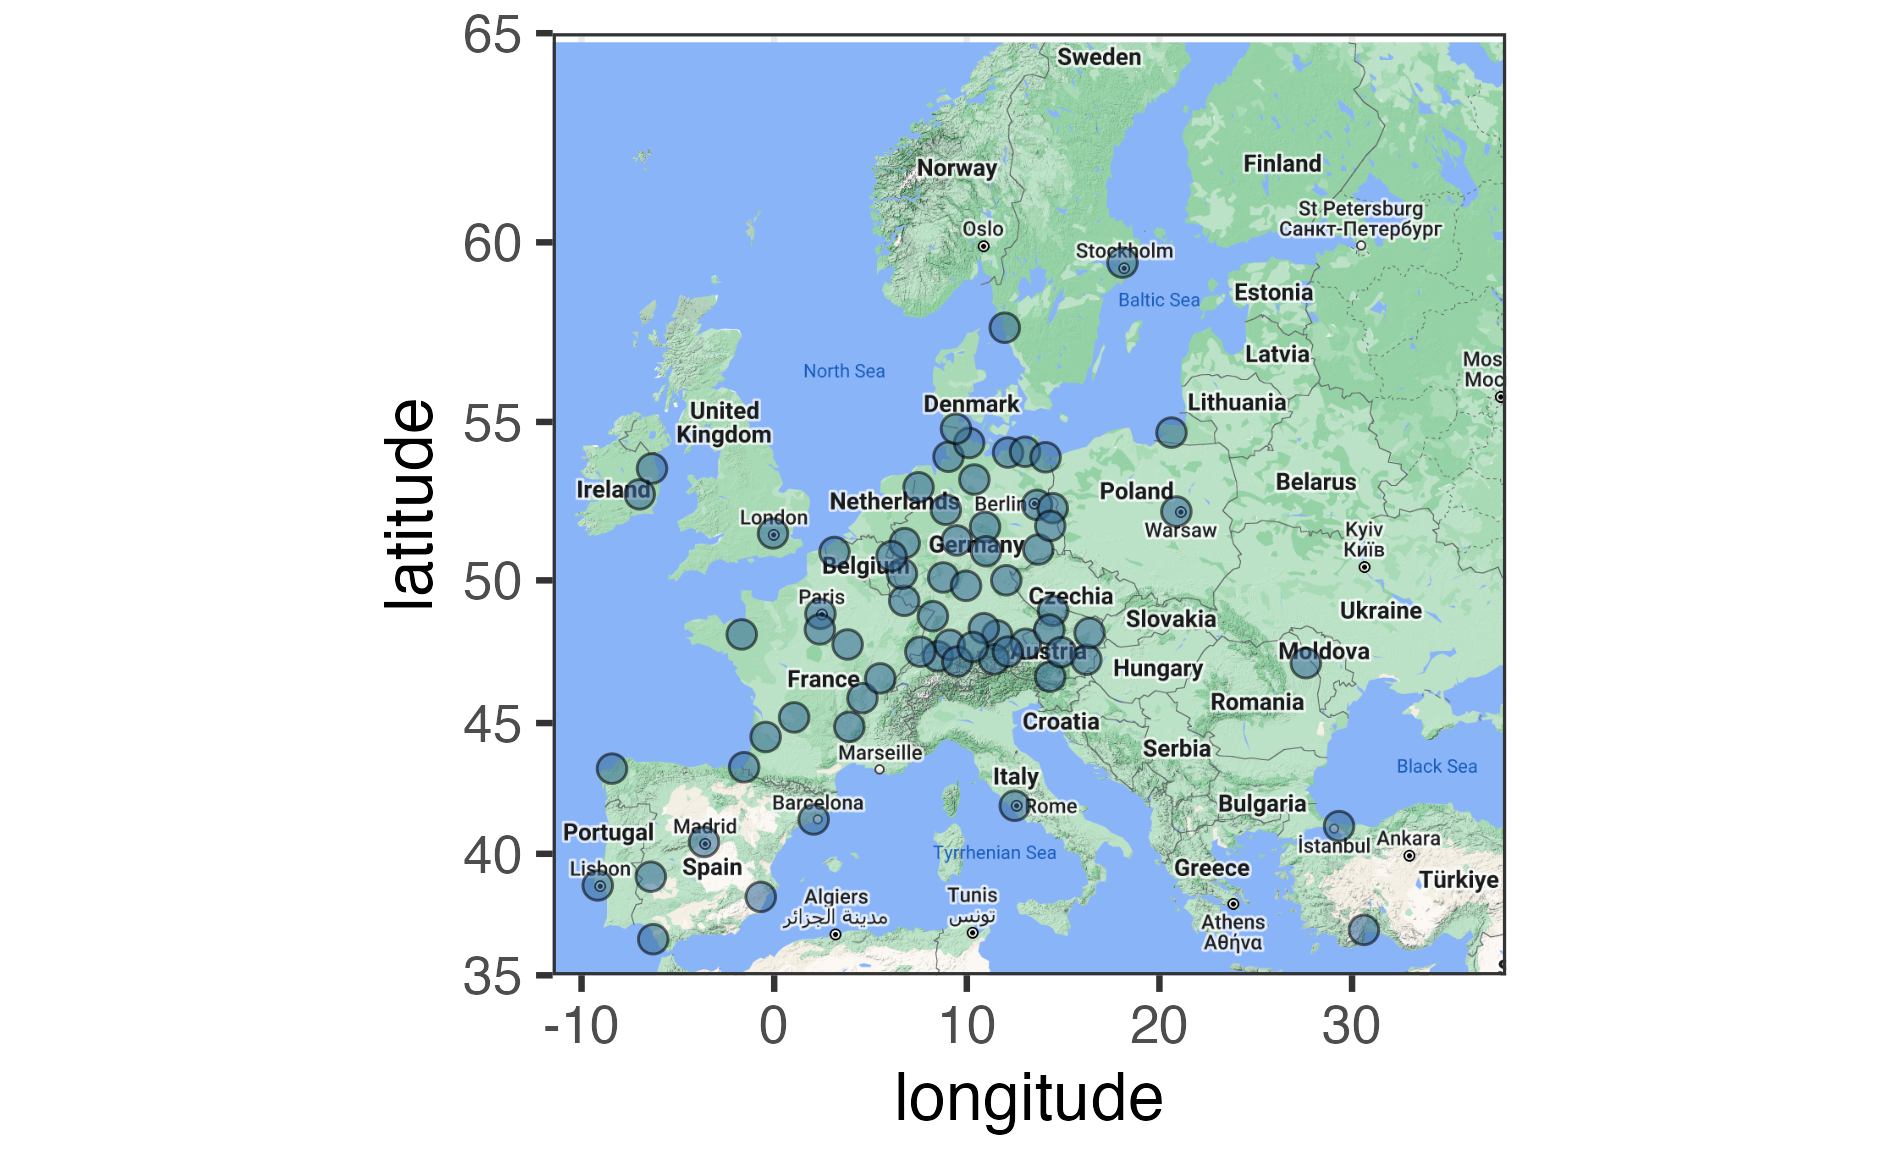
\includegraphics{../plots/map.png}
  \caption{Geographical distribution of water analysis reports included in the source water dataset. Green: analysis of municipal tap water; Red: rainwater analysis.}
  \label{fig:map_water}
\end{figure}

It is common practice to report the value of the detection limit instead
of the measured value in case that the analyte concentration found was
below the sensitivity of the instrument used for measurement (Deutsches
Institut für Normung e.V. 2008). Figure 2.3 shows the proportion of data
for all considered analytes in the water analysis reports that were
found to be below the detection limit. Retaining the detection limits in
the dataset leads to mean concentration estimates that are too high.
Therefore, concentration data was recalculated using the \emph{cenmle()}
function from the R package NADA by \gls{mle} (Helsel 2011). This
ensured that the estimates for nutrient concentrations in tap water were
reliable. The output was eventually used to calculate the two-sided
\SI{90}{\p} confidence interval for the arithmetic mean of the
concentration of each nutrient to describe the concentration range that
will be found in \SI{90}{\p} of all cases where tap water is used.
Finally, multiplying the obtained concentrations with AWE yielded the
upper and lower limits of the \SI{90}{\p} confidence interval of total
daily individual plant nutrient inputs via source water.

\hypertarget{aquafeeds}{%
\subsubsection{Aquafeeds}\label{aquafeeds}}

The daily feed input resulting from the rearing assumptions was 482.5
\si{\kg\per\d}.

In the third step, daily nutrient inputs via aquafeeds were estimated.
The IDS was filtered for studies reporting the name of the commercial
aquafeed used (if not selfmade), the CP inclusion rate and the feeding
rate. From the resulting FDS2, the average feeding rate (\(FR\);
\si{\p}), CP inclusion rate (ACP) and the averages of all plant
nutrients were calculated. Due to lacking nutrient composition data,
supplier datasheets were used and amended by literature data in case of
utilization of commercial aquafeeds. Incomplete observations with
respect to experimental feeds were handled in the same way, merging data
from multiple publications if the same feed was used. NA values were
removed for the computation of averages. Eventually, the average daily
feed input (\(FI\); \si{\kg\per\d}) was calculated by multiplying ABM
from the generated system assumptions with XXXXX. By multiplying \(FI\)
with the average plant nutrient inclusion rates in the aquafeeds, the
uncorrected total daily input of individual plant nutrients via
aquafeeds could be calculated. Obtained values were then corrected by
multiplication with apparent digestibility coefficients (ADC),
accounting for the digestibility of aquafeeds by fish. An ADC of
\SI{90}{\p} was assumed for N whereas the ADC of all other nutrients was
assumed to be \SI{50}{\p} (\textbf{Lall2002?}). Finally, it was assumed
that \SI{50}{\p} of the digestible fraction is retained while the
remaining \SI{50}{\p} is excreted in dissolved form (Halver and Hardy
2003). The indigestible part of the feed is excreted as solid feces and
was thus assumed not to participate in chemical reactions in solution.
Lastly, an estimate for the daily input of alkalinity supplements was
derived from \(AFI\). First, the daily CP input was calculated by
multiplying \(AFI\) with the percentage of \(CP\) on dry matter basis in
the feed.

\hypertarget{software}{%
\subsection{Software}\label{software}}

All calculations were conducted using R (v4.2.2) with RStudio (``Spotted
Wakerobin'' Release) as graphical user interface.

\hypertarget{aquafeeds-as-nutrient-sources}{%
\section{Aquafeeds as nutrient
sources}\label{aquafeeds-as-nutrient-sources}}

Aquafeeds are considered to be the most important source of nutrients,
providing a large and continuous nutrient input into the system.
Formulating a specific aquaponics feed was thus thought to be the most
suitable approach to develop an ``off-the-shelf'' nutrient delivery
system (Lennard 2017; Eck, Körner, and Jijakli 2019). When discussing
aquafeeds as nutrient input route, it is important to consider pathways
of diet utilization, as shown in Figure 1.2. Uneaten feed and the
indigestible mass fraction of ingested feed make up the solid wastes.
The digestible mass fraction is meanwhile utilized to sustain the
animals' basal metabolism, somatic growth and reproductive activity.
Metabolic end products are then excreted via the gills and the urinary
system in form of dissolved matter (\textbf{Hardy2003?}; Evans,
Piermarini, and Choe 2005). Only the dissolved fraction of the nutrients
is immediately available for plant uptake via the root system.

The availability of digestibility, retentiton and excretion data for
individual nutrients, with the former expressed as \gls{adc}, depends on
whether the nutrient is essential and has to be considered for feed
formulation.

N that is, for the most part, present as \gls{cp} in aquafeeds, is
generally well-digestible, with an \gls{adc} usually being above
\SI{70}{\p} and on average approximately \SI{90}{\p} (Guillaume et al.
2001; International Aquaculture Feed Formulation Database (IAFFD) 2021).
The excretion of N as end product of the protein and amino acid
catabolism takes place in form of ammonia (\ce{NH3}) and, to a small
extent, urea. The predominant excretory site are the gills, followed by
renal excretion (Dabrowski and Guderley 2003).

A less digestible nutrient is P with \gls{adc} ranging from \SI{70}{\p}
to only \SI{40}{\p} and a resulting excretion of \SI{30}{\p} to
\SI{60}{\p} of the supply (Lall 2003; Sugiura 2018). Especially plant
ingredients in aquafeeds can cause low \gls{adc} if they are rich in
phytic acid. Phytic acid is poorly digestible and can furthermore reduce
the digestibility of minerals in the feed. This might also explain
contradictory information in literature with reported renal excretion
rates of \SI{90}{\p} of the total excreta (Lall 2003) in contrast to
estimates of \SI{28}{\p} of excretion taking place in dissolved form and
\SI{30}{\p} to \SI{64}{\p} excreted as particulate P (Dabrowski and
Guderley 2003).

Studies about \gls{adc} for the remaining essential plant nutrients are
scarce. Variability of \gls{adc} among different feed ingredients was
shown in Atlantic salmon (\emph{Salmo salar}) for Ca, Mg, Fe, Mn and Zn,
with \gls{adc} ranging between \SIrange{30}{50}{\p} (Sugiura et al.
1998). Excretion of the earth alkaline metals Ca and Mg primarily occurs
in dissolved form via the gills and urine (Oikari and Rankin 1985; Lall
2003). Mn, in contrast, is mostly excreted in solid form as feces, while
renal excretion was found to be negligible (Lall 2003). Cu is
predominantly excreted via the bile (Bury, Walker, and Glover 2003).
Excess dietary Cu is not taken up but excreted as feces. Cu inclusion
rates in aquafeeds are thus reduced to minimize its release into the
environment (Lall 2003). Excretion of Zn mostly takes place renally and
via the gills (Lall 2003).

\hypertarget{water-as-nutrient-source}{%
\section{Water as nutrient source}\label{water-as-nutrient-source}}

\begin{itemize}
\tightlist
\item
  Why is water added?
\item
  Where does it come from?
\end{itemize}

Water is added to the system either to compensate evaporation, spillage
or leaning losses (e.g., the drum filter backwash) or to dilute
accumulating substances such as nitrate. The source water can originate
from wells, collected rain or the municipal tap.

Meanwhile, the importance of water as nutrient source is seen as
negligible (Schmautz et al. 2016). However, large amounts of calcium
(Ca), magnesium (Mg) and sulfur (S), that are essential plant nutrients,
were found to enter the system via exchange water in one study (Delaide
et al. 2017).

A recent survey revealed that the majority of European aquaponics
entities (\SI{71.7}{\p}) uses municipal tap water
(\textbf{Raulier2023?}). Aquaponic food production is usually seen in
the context of decentralized urban farming, where limited space due to
high land prices is compensated by innovative approaches such as
vertical farming and synergy effects due to the simultaneous production
of fish and crops. Though, it has to be considered that the availability
of rain water and space for its storage is limited and wells are
unlikely to be approved by authorities. Thus, tap water would

This observation will likely

This is not surprising, considering that aquaponic facilities

Though, water can vary in its composition, depending on its origin. A
glimpse of the extent of variability of terrestrial waters in their
chemical composition is provided in Figure 1.1. Weathering of rock, ion
exchange, redox reactions and the buildup of biomass are the main
processes that are affecting concentrations of the shown compounds
(Stumm 1981). The highest variability can be found in anionic compounds
such as nitrate (\ce{NO3-}) and sulfate (\ce{SO4^2-}) and the cationic
alkaline earth metals \ce{Ca^2+} and \ce{Mg^2+} that are covering a
concentration range of approximately two orders of magnitude.

\hypertarget{alkalinity-supplements-as-nutrient-sources}{%
\section{Alkalinity supplements as nutrient
sources}\label{alkalinity-supplements-as-nutrient-sources}}

The term alkalinity supplements summarizes several alkaline substances
that are used to maintain a stable pH in the water (Timmons 2010).
Nitrification decreases the pH over time and, consequently, also the
activity of nitrifyers {[}Ward2011{]}. Thus, a stable pH has to be
maintained to ensure both high nitrification performance and animal
welfare. For this purpose, several Na-based substances such as sodium
hydrogen carbonate (baking soda, \ce{NaHCO3}) are commonly used in
aquaculture due to their high and rapid solubility at a comparably cheap
price. However, high sodium (Na) concentrations must be avoided in
aquaponic systems due to its phytotoxicity (Maathuis, Ahmad, and
Patishtan 2014). Na is therefore replaced with several other supplements
based on K or Ca that come with the benefit of providing an additional
source of nutrients besides increasing the pH.

\hypertarget{contribution-of-the-nutrient-sources-to-the-total-nutrient-mass-flows}{%
\section{Contribution of the nutrient sources to the total nutrient mass
flows}\label{contribution-of-the-nutrient-sources-to-the-total-nutrient-mass-flows}}

The average nutrient composition of both aquafeeds and source water and
the lower and upper limits of the \SI{90}{\p} confidence interval for
source water are shown in Table 3.1. Figure 3.2 provides an additional
graphical presentation of the findings with emphasis on the variability
of nutrient contributions by source water.

The highest daily nutrient inputs with respect to the macronutrients N
and P in the reviewed studies likely originated from aquafeeds, being on
average 99.2\% and 99.3\%, respectively. The overall amounts of these
two nutrients contributed by source water are negligible. Aquafeeds can
also be assumed being the main source of the micronutrients Fe, Mn, Cu,
Zn, and Mo, with an average contribution of 96.2\%, 97.2\%, 79.8\%,
93.9\% and 76.3\%, respectively. Among these nutrients, Cu and Mo showed
the highest variability with respect to the contribution of source water
between locations (Cu 90\% CI: 8\%, 29.7\%; Mo 90\% CI: 14.7\%, 29.3\%),
with up to almost a third of the daily inputs possibly entering the
system via the water. Meanwhile, source water likely had a comparably
high contribution to Mg and S. With 76.5\% for Mg (90\% CI: 72.1\%,
79.7\%) and 68.8\% for S (90\% CI: 58.9\%, 74.8\%), an average delivery
of more than half of the daily input was found. Also, a considerable
contribution to daily B (63.1\%; 90\% CI: 48.5\%, 48.5\%) and Ni
(56.2\%; 90\% CI: 33.3\%, 67.4\%) inputs probably originated from the
source water.

Inputs of the remaining two nutrients, K and Ca, were found to be
heavily depending on the alkalinity supplement used. In absence of the
alkalinity supplement, aquafeeds were found to have the greatest impact
on K with a contribution of 81.16\%, while a higher proportion of Ca
(69.62\%; 90\% CI: 65.51\%, 72.86\%) would enter the system on average
via the water, compared with an average of30.38\% of feed contribution.
The difference is more pronounced with respect to Na: 82.25\% (90\% CI:
73.11\%, 86.76\%) of the total input was calculated to originate from
water while only 17.75\% were found to enter the system via daily
feeding. However, the calculated quantities of alkalinity supplements
necessary to maintain a constant pH were found to dominate each input
scenario, resulting in a contribution of more than 80\% of the total
input of K, Ca, or Na in any case.

\hypertarget{economic-considerations}{%
\subsection{Economic considerations}\label{economic-considerations}}

Table 3.2 summarizes some supplements, their properties and prices.
Using one of these substances would result in the supplement
contributing 98.7\%, 86.5\% or 96.3\% of the total K, Ca or Na input,
respectively. Regarding the costs for alkalinity supplements, Na based
substances are the cheapest, with prices of between 0.01 and 0.03 EUR
d-1, followed by Ca based supplements ranging in the same price class.
The most expensive supplements to be used are those based on K. These
substances would cause costs between 0.10 and 0.14 EUR d-1, thus being
on average 6 times more expensive than Ca or Na based substances.

The contribution of different nutrient sources to the total daily
nutrient inputs into an aquaponic system were compared based on
assumptions derived from literature. It could overall be confirmed by
the current input scenario that aquafeeds serve as major nutrient input
route for N, P, K, Fe, Mn, Cu, Zn, and Mo after consideration of
digestibility and nutrient retention by fish. These results confirm
prior findings (Delaide et al. 2017). Considering variability among
locations, it could furthermore be confirmed that Ca, Mg, S, B and Na
originate from source water. However, the variability found in the case
of Ca does not reflect the usual concentration range of approximately
two orders of magnitude found in terrestrial waters (Stumm 1981). A
study reviewing the Ca concentration in tap waters from the USA and
Canada found a range from \SIrange{1}{135}{\mgL} (Morr et al. 2006).

Considering that the obtained results were obtained making use of
assumptions, these initial assumptions need to be discussed. The species
distribution with strong emphasis on Tilapia (\emph{Oreochromis} spp.)
and African catfish (\emph{Clarias gariepinus}) matches with survey
results obtained in Europe (Villarroel et al. 2016), even though
approximately half of the studies included in the dataset were conducted
in the USA. However, surveys conducted in the USA also revealed that the
species mostly cultivated in aquaponic systems are Tilapia (Love et al.
2015; Pattillo et al. 2022). On the other hand, the average stocking
density of 7.69 kg m-3 that was used for the nutrient contribution
calculations can neither be considered representative for the intensive
cultivation of Tilapia nor for African catfish. While densities between
\SIrange{10}{50}{\kg\per\cubicm} are reported as acceptable for
cultivation in RAS systems (\textbf{El-Sayed2019?}), densities of
\SI{120}{\kg\per\cubicm} were reported to be tolerated by the latter
species without any adverse effects on fish health (Nieuwegiessen et al.
2009). Even though salmonids such as Rainbow trout
(\emph{Oncorhynchus mykiss}) are seldom reared in aquaponic systems,
they can tolerate stocking densities up to \SI{137}{\kg\per\cubicm}.
Though, normal stocking densities range between
\SIrange{10}{20}{\kg\per\cubicm}. The assumptions are rather on the
lower end for salmonids (Pennell and McLean 1996). Common carp
(\emph{Cyprinus carpio}) is irrelevant for aquaponic systems due to its
low market price. Though, it was found that fish welfare can be
guaranteed at a stocking density of around \SI{28}{\kg\per\cubicm},
which is \(\approx 4\) times higher than the assumed density (Ruane,
Carballo, and Komen 2002). Consequently, it can be expected that the
contribution of aquafeeds to the total daily nutrient input under
intensive rearing conditions for the mentioned fish species is
considerably higher than assumed in this study. Though, the presented
nutrient contribution scenario might be representative for the
cultivation of Pikeperch due to the comparably low stocking densities
(\(\approx\)\SI{5}{\kg\per\cubicm}) recommended for its cultivation
(Kestemont, Dabrowski, and Summerfelt 2015). The average \gls{fr} of
\SI{2}{\p} is in line with recommendations for the husbandry of Tilapia,
Channel catfish (Ictalurus punctatus) and Common carp (Lovell 2003).
Another aspect with respect to the contribution of feeds is that the
feed composition is, in adaptation to the species to be reared,
variable. For instance, crude protein inclusion rates in commercial
aquafeeds for the mentioned species range from 32\% for O. spp. (Wilson
2003; \textbf{El-Sayed2019?}) to \SI{50}{\p} for Pikeperch (Geay and
Kestemont 2015). Further variation in the nutrient composition is
introduced by feed manufacturers due to changes in its raw material
composition made because of fluctuations in feed ingredient availability
and market prices. While changes in the mass concentrations of crucial
nutrients such as the \gls{cp} inclusion rate are acceptable only within
tight limits, this might not be the case for other nutrients that are
disregarded in the formulation process. Overall, data about the
inclusion rates of nutrients relevant for plants in commercial aquafeeds
can be considered scarce because these compounds are either not
essential for aquatic animals or can be taken up from water via the
gills in sufficient quantities. These nutrients are thus usually not
considered during feed formulation (Lall 2003). However, a comprehensive
review about the range of plant nutrient mass concentrations in
commercial aquafeeds has not yet been conducted to the best of the
authors knowledge. The mean water exchange rate of 3\% can be considered
at the lower end of commonly reported water exchange rates for RAS and
within the range recommended for aquaponic systems (Timmons 2010).

Using analysis reports from municipal water suppliers can be considered
as valid approach with respect to the acquisition of nutrient
concentration data in source water as it was found by a prior survey
that educators, including research institutions, usually use tap water
(Love et al. 2015). It could be further argued that, due to its low
water demand, aquaponics is generally seen as food production system
suitable for urban areas or arid regions (Kloas et al. 2015; Joyce et
al. 2019). Establishing an aquaponic system in these regions comes with
limited access to water sources such as well water or rivers and lakes.
Rainwater, on the other hand, would require large storage capacities.
Tap water is thus assumed to be the most important water source.
Recalculation of nutrient concentrations as response to high proportions
of censored data where only the limit of detection is reported is a
rather uncommon approach. However, removing the affected observations
would have resulted in a loss of a large proportion of data and, in
addition, would have led to an average value that is higher than the
estimates obtained by recalculation because the remaining data consisted
only of concentration values that are high enough to be determined. A
similar result would have arisen from using the reported detection
limits for the calculation of nutrient concentration means. The results
of the nutrient concentration recalculation via MLE procedure can thus
be considered closer to the true concentration means than the outcome of
the other mentioned approaches.

The daily quantity of alkalinity supplements to be added might be
overestimated. In biofilters, both nitrification and denitrification
processes usually occur due to partially anoxic conditions, for instance
within biofilms. Denitrification yields alkalinity (Timmons 2010).
However, the contribution of alkalinity supplements will likely still
exceed 50\% of the total daily nutrient inputs. Furthermore, the
calculations assumed that the supplements would have a purity of 100\%.
In practice a lower purity, corresponding to a food grade certification,
can be expected.

\hypertarget{implications-for-the-formulation-of-tailored-aquaponics-feeds}{%
\subsection{Implications for the formulation of tailored aquaponics
feeds}\label{implications-for-the-formulation-of-tailored-aquaponics-feeds}}

Firstly, considering potential precipitation, target nutrients for an
increased delivery could include N, K, Mg, S, B, and Zn. This suggestion
is partly confirmed by prior empirical studies. One of those found K,
Mg, and Zn to accumulate out of the mentioned nutrients, with additional
accumulation of P, Mn and Zn (Seawright, Stickney, and Walker 1998).
Another study reported N, K, and Mg accumulation alongside P and Cu
(Shaw et al.~2022). The focus on K and Mg can thus be considered
``safe'', considering the generally high solubility of both compounds
(Lide 2007) and reported deficiencies for both in aquaponics (Lunda et
al. 2019). Natural feed ingredients rich in K are soy lecithin
(\SI{13.0}{\p} K on dry matter basis), vinasse (\SI{3.6}{\p} K on dry
matter basis) and some protein feedstuffs such as poultry by-product
meal (\SI{3.5}{\p} K on dry matter basis) and hydrolyzed fish solubles
\SIrange{2.4}{2.9}{\p} K on dry matter basis). Mg can be introduced to
aquafeeds mostly via the use of seaweed (\SI{3.9}{\p} Mg on dry matter
basis) (International Aquaculture Feed Formulation Database (IAFFD)
2021). The drawback of the use of some of the above-stated feed
ingredients is that the target nutrient is usually accompanied by
comparably high amounts of Na. Even though this study shows that
aquafeeds were not the main input route of Na in the reviewed
literature, it is nevertheless reasonable to attempt to decrease Na
inclusion rates during feed formulation because the initial assumptions
leading to the nutrient input scenarios are not representative for
commercial systems, as described above. This could be done for instance
by replacement of feed ingredients with high Na inclusion rates such as
fish meal originating from marine fish by other protein feedstuffs.

Another possibility is given by using food-grade salts of the desired
nutrients. However, considering the nutrient input via feed
(\SI{1.1}{\p}) in comparison with that of alkalinity supplements
containing K (\SI{98.7}{\p}) in this study, it depends on target
concentrations and costs whether it is reasonable or not to increase the
inclusion rate of K in a tailored aquafeed versus using the respective
alkalinity supplements.

It remains questionable whether it is more meaningful to include, for
instance, salts into the feed or to add them directly into the system.
Inclusion rates of nutrients that are confirmed to be affected by
precipitation (Ca, Fe) are, in turn, recommended to be decreased in case
the nutrient is not essential for the livestock and a change in feed
formulation economically viable.

\hypertarget{conclusion}{%
\section{Conclusion}\label{conclusion}}

This article provides a synthesis of information concerning the sources
of nutrients in aquaculture and aquaponic systems, their contribution to
the total daily nutrient mass flows and their variability.

\hypertarget{references}{%
\section*{References}\label{references}}
\addcontentsline{toc}{section}{References}

\hypertarget{refs}{}
\begin{CSLReferences}{1}{0}
\leavevmode\vadjust pre{\hypertarget{ref-Bury2003}{}}%
Bury, Nicolas R., Paul A. Walker, and Chris N. Glover. 2003.
{``Nutritive Metal Uptake in Teleost Fish.''} \emph{Journal of
Experimental Biology} 206 (1): 11--23.
\url{https://doi.org/10.1242/jeb.00068}.

\leavevmode\vadjust pre{\hypertarget{ref-Dabrowski2003}{}}%
Dabrowski, Konrad, and Helga Guderley. 2003. {``{Intermediary
Metabolism}.''} In \emph{Fish Nutrition}, 3rd ed., 309--65. Elsevier
Science.

\leavevmode\vadjust pre{\hypertarget{ref-Delaide2017}{}}%
Delaide, Boris, Guillaume Delhaye, Michael Dermience, James Gott, Hélène
Soyeurt, and M. Haissam Jijakli. 2017. {``Plant and Fish Production
Performance, Nutrient Mass Balances, Energy and Water Use of the {PAFF}
Box, a Small-Scale Aquaponic System.''} \emph{Aquacultural Engineering}
78: 130--39. \url{https://doi.org/10.1016/j.aquaeng.2017.06.002}.

\leavevmode\vadjust pre{\hypertarget{ref-Eck2019}{}}%
Eck, Mathilde, Oliver Körner, and M. Haïssam Jijakli. 2019. {``{Nutrient
Cycling in Aquaponics Systems}.''} In \emph{Aquaponics Food Production
Systems}, 231--46. Springer International Publishing.
\url{https://doi.org/10.1007/978-3-030-15943-6_9}.

\leavevmode\vadjust pre{\hypertarget{ref-Evans2005}{}}%
Evans, David H., Peter M. Piermarini, and Keith P. Choe. 2005. {``The
Multifunctional Fish Gill: Dominant Site of Gas Exchange,
Osmoregulation, Acid-Base Regulation, and Excretion of Nitrogenous
Waste.''} \emph{Physiological Reviews} 85 (1): 97--177.
\url{https://doi.org/10.1152/physrev.00050.2003}.

\leavevmode\vadjust pre{\hypertarget{ref-Geay2015}{}}%
Geay, Florian, and Patrick Kestemont. 2015. {``Feeding and Nutrition of
Percid Fishes During Ongrowing Stages.''} In \emph{Biology and Culture
of Percid Fishes}, 587--622. Springer Netherlands.
\url{https://doi.org/10.1007/978-94-017-7227-3_22}.

\leavevmode\vadjust pre{\hypertarget{ref-Guillaume2001}{}}%
Guillaume, Jean, Sadasivam Kaushik, Pierre Bergot, and Robert Metailler.
2001. \emph{Nutrition and Feeding of Fish and Crustaceans (Springer
Praxis Books / Food Sciences)}. Springer.

\leavevmode\vadjust pre{\hypertarget{ref-Halver2003}{}}%
Halver, John E., and Ronald W. Hardy. 2003. {``Nutrient Flow and
Retention.''} In \emph{Fish Nutrition}, 755--70. Elsevier.
\url{https://doi.org/10.1016/B978-012319652-1/50015-X}.

\leavevmode\vadjust pre{\hypertarget{ref-Helsel2011}{}}%
Helsel, Dennis R. 2011. {``Statistics for Censored Environmental Data
Using Minitab{\textregistered} and r,''} December.
\url{https://doi.org/10.1002/9781118162729}.

\leavevmode\vadjust pre{\hypertarget{ref-IAFFD2021}{}}%
International Aquaculture Feed Formulation Database (IAFFD). 2021.
{``{Feed Ingredients Composition Database (FICD) v7.0}.''}
\url{https://app.iaffd.com}.

\leavevmode\vadjust pre{\hypertarget{ref-Joyce2019}{}}%
Joyce, Alyssa, Mike Timmons, Simon Goddek, and Timea Pentz. 2019.
{``{Bacterial Relationships in Aquaponics: New Research Directions}.''}
In \emph{Aquaponics Food Production Systems}, 145--61. Springer
International Publishing.
\url{https://doi.org/10.1007/978-3-030-15943-6_6}.

\leavevmode\vadjust pre{\hypertarget{ref-Kestemont2015}{}}%
Kestemont, Patrick, Konrad Dabrowski, and Robert C. Summerfelt, eds.
2015. {``Biology and Culture of Percid Fishes.''}
\url{https://doi.org/10.1007/978-94-017-7227-3}.

\leavevmode\vadjust pre{\hypertarget{ref-Kloas2015}{}}%
Kloas, W, R Groß, D Baganz, J Graupner, H Monsees, U Schmidt, G Staaks,
et al. 2015. {``A New Concept for Aquaponic Systems to Improve
Sustainability, Increase Productivity, and Reduce Environmental
Impacts.''} \emph{Aquaculture Environment Interactions} 7 (2): 179--92.
\url{https://doi.org/10.3354/aei00146}.

\leavevmode\vadjust pre{\hypertarget{ref-Lall2003}{}}%
Lall, Santosh P. 2003. {``{The Minerals}.''} In \emph{Fish Nutrition},
3rd ed., 259--308. Elsevier Science.

\leavevmode\vadjust pre{\hypertarget{ref-Lennard2017}{}}%
Lennard, Wilson. 2017. \emph{Commercial Aquaponic Systems: Integrating
Recirculating Fish Culture with Hydroponic Plant Production}. Victoria,
Australia: Wilson Lennard.

\leavevmode\vadjust pre{\hypertarget{ref-Lide2007}{}}%
Lide, David R. 2007. \emph{{CRC Handbook of Chemistry and Physics}}.
88th ed. CRC Press.

\leavevmode\vadjust pre{\hypertarget{ref-Love2015}{}}%
Love, David C., Jillian P. Fry, Ximin Li, Elizabeth S. Hill, Laura
Genello, Ken Semmens, and Richard E. Thompson. 2015. {``Commercial
Aquaponics Production and Profitability: Findings from an International
Survey.''} \emph{Aquaculture} 435: 67--74.
\url{https://doi.org/10.1016/j.aquaculture.2014.09.023}.

\leavevmode\vadjust pre{\hypertarget{ref-Lovell2003}{}}%
Lovell, Richard T. 2003. {``Diet and Fish Husbandry.''} In \emph{Fish
Nutrition}, 3rd ed., 703--54. Elsevier Science.

\leavevmode\vadjust pre{\hypertarget{ref-Lunda2019}{}}%
Lunda, Roman, Koushik Roy, Jan Másílko, and Jan Mráz. 2019.
{``Understanding Nutrient Throughput of Operational {RAS} Farm Effluents
to Support Semi-Commercial Aquaponics: Easy Upgrade Possible Beyond
Controversies.''} \emph{Journal of Environmental Management} 245:
255--63. \url{https://doi.org/10.1016/j.jenvman.2019.05.130}.

\leavevmode\vadjust pre{\hypertarget{ref-Maathuis2014}{}}%
Maathuis, Frans J. M., Izhar Ahmad, and Juan Patishtan. 2014.
{``Regulation of \(\text{Na}^{+}\) Fluxes in Plants.''} \emph{Frontiers
in Plant Science} 5 (September).
\url{https://doi.org/10.3389/fpls.2014.00467}.

\leavevmode\vadjust pre{\hypertarget{ref-Morr2006}{}}%
Morr, Simon, Esteban Cuartas, Basil Alwattar, and Joseph M. Lane. 2006.
{``How Much Calcium Is in Your Drinking Water? A Survey of Calcium
Concentrations in Bottled and Tap Water and Their Significance for
Medical Treatment and Drug Administration.''} \emph{{HSS}
Journal{\textregistered}: The Musculoskeletal Journal of Hospital for
Special Surgery} 2 (2): 130--35.
\url{https://doi.org/10.1007/s11420-006-9000-9}.

\leavevmode\vadjust pre{\hypertarget{ref-Nieuwegiessen2009}{}}%
Nieuwegiessen, Pascal G. van de, Jacob Olwo, Sophoan Khong, Johan A. J.
Verreth, and Johan W. Schrama. 2009. {``Effects of Age and Stocking
Density on the Welfare of African Catfish, Clarias Gariepinus
Burchell.''} \emph{Aquaculture} 288 (1-2): 69--75.
\url{https://doi.org/10.1016/j.aquaculture.2008.11.009}.

\leavevmode\vadjust pre{\hypertarget{ref-Oikari1985}{}}%
Oikari, A. O., and J. C. Rankin. 1985. {``Renal Excretion of Magnesium
in a Freshwater Teleost, \emph{Salmo Gairdneri}.''} \emph{Journal of
Experimental Biology} 117 (1): 319--33.
\url{https://doi.org/10.1242/jeb.117.1.319}.

\leavevmode\vadjust pre{\hypertarget{ref-Pattillo2022}{}}%
Pattillo, D. Allen, Janelle V. Hager, David J. Cline, Luke A. Roy, and
Terrill R. Hanson. 2022. {``System Design and Production Practices of
Aquaponic Stakeholders.''} Edited by Pramod K Pandey. \emph{{PLOS}
{ONE}} 17 (4): e0266475.
\href{https://doi.org/10.1371/journal.\%20pone.0266475}{https://doi.org/10.1371/journal.
pone.0266475}.

\leavevmode\vadjust pre{\hypertarget{ref-Pennell1996}{}}%
Pennell, William, and William E. McLean. 1996. {``Early Rearing.''} In
\emph{Principles of Salmonid Culture}, edited by William Pennell and
Bruce A. Barton, 365--465. Elsevier B.V.

\leavevmode\vadjust pre{\hypertarget{ref-Rakocy2006}{}}%
Rakocy, James E., Michael P. Masser, and Thomas M. Losordo. 2006.
{``Recirculating Aquaculture Tank Production Systems: Aquaponics -
Integrating Fish and Plant Culture.''} In \emph{Southern Regional
Aquaculture Center (SRAC) Publications}. Vol. 454. Oklahoma State
University.

\leavevmode\vadjust pre{\hypertarget{ref-Robaina2019}{}}%
Robaina, Lidia, Juhani Pirhonen, Elena Mente, Javier Sánchez, and Neill
Goosen. 2019. {``{Fish Diets in Aquaponics}.''} In \emph{Aquaponics Food
Production Systems}, 333--52. Springer International Publishing.
\url{https://doi.org/10.1007/978-3-030-15943-6_13}.

\leavevmode\vadjust pre{\hypertarget{ref-Ruane2002}{}}%
Ruane, N. M., E. C. Carballo, and J. Komen. 2002. {``{Increased stocking
density influences the acute physiological stress response of common
carp \emph{Cyprinus carpio} ( L.)}.''} \emph{Aquaculture Research} 33:
777--84.

\leavevmode\vadjust pre{\hypertarget{ref-Schmautz2016}{}}%
Schmautz, Zala, Fionna Loeu, Frank Liebisch, Andreas Graber, Alex
Mathis, Tjaša Griessler Bulc, and Ranka Junge. 2016. {``Tomato
Productivity and Quality in Aquaponics: Comparison of Three Hydroponic
Methods.''} \emph{Water} 8 (11): 533.
\url{https://doi.org/10.3390/w8110533}.

\leavevmode\vadjust pre{\hypertarget{ref-Seawright1998}{}}%
Seawright, Damon E., Robert R. Stickney, and Richard B. Walker. 1998.
{``Nutrient Dynamics in Integrated Aquaculture-Hydroponics Systems.''}
\emph{Aquaculture} 160: 215--37.

\leavevmode\vadjust pre{\hypertarget{ref-Stumm1981}{}}%
Stumm, Werner. 1981. \emph{Aquatic Chemistry: Chemical Equilibria and
Rates in Natural Waters}. 3rd ed. Wiley.

\leavevmode\vadjust pre{\hypertarget{ref-Sugiura2018}{}}%
Sugiura, Shozo H. 2018. {``Phosphorus, Aquaculture, and the
Environment.''} \emph{Reviews in Fisheries Science and Aquaculture} 26
(4): 515--21. \url{https://doi.org/10.1080/23308249.2018.1471040}.

\leavevmode\vadjust pre{\hypertarget{ref-Sugiura1998}{}}%
Sugiura, Shozo H., Faye M. Dong, Cindra K. Rathbone, and Ronald W.
Hardy. 1998. {``Apparent Protein Digestibility and Mineral
Availabilities in Various Feed Ingredients for Salmonid Feeds.''}
\emph{Aquaculture} 159: 177--202.

\leavevmode\vadjust pre{\hypertarget{ref-Timmons2010}{}}%
Timmons, M. B. 2010. \emph{Recirculating Aquaculture: 2nd Edition}.
Cayuga Aqua Ventures.

\leavevmode\vadjust pre{\hypertarget{ref-Villarroel2016}{}}%
Villarroel, Morris, Ranka Junge, Tamas Komives, Bettina König, Ignacio
Plaza, András Bittsánszky, and Agnès Joly. 2016. {``Survey of Aquaponics
in Europe.''} \emph{Water} 8 (10): 468.
\url{https://doi.org/10.3390/w8100468}.

\leavevmode\vadjust pre{\hypertarget{ref-Wilson2003}{}}%
Wilson, Robert P. 2003. {``{Amino Acids and Proteins}.''} In \emph{Fish
Nutrition}, Third, 143--79. Elsevier Science.
\url{https://doi.org/10.1016/b978-012319652-1/50004-5}.

\end{CSLReferences}


\end{document}
